%!TeX spellcheck = en_GB
% Die erste (unkommentierte) Zeile im Dokument legt immer die
% Dokumentklasse fest
\documentclass{scrartcl} 

% Präambel:
% Einbinen von zusätzlichen Paketen. Falls für eine Datei keine Endung
% explizit angegeben wird, benutzt LaTeX '.tex'. Im Folgenden wird
% also die Datei 'edv_pakete.tex' eingebunden.
\input{edv_pakete}


% Verzeichnisse mit Abbildungen; kann gestrichen werden,
% falls Sie dies schon in edv_pakete.tex definiert haben:
%\graphicspath{{../report}}

\addbibresource{refs.bib} %Hinzufügen einer Literaturdatenbank aus dem angegebenen Verzeichnis

% Titel, Autor und Datum
\title{Computational Physics}
\subtitle{Exercise 6}
\date{\today}
\author{Christiane Groß, Nico Dichter}

% Jetzt startet das eigentliche Dokument
\begin{document}
	\maketitle
	
\section{Theory}
The following relations were given on the exercise sheet. And should be assumed, that both particles have the same mass: $m_1=m_2=m=m_N$
\begin{align}
	\bra{\vec{k}_1'}\rho(\vec{q})\ket{\vec{k}_1}&=\delta(\vec{k}_1'-\vec{q}-\vec{k}_1)\label{eq:rhok}\\
	\bra{\Psi \vec{P}'}\rho(\vec{q})\ket{\Psi\vec{P}}&=F(\vec{q}^2)\delta(\vec{P}'-\vec{q}-\vec{P})\label{eq:rhopsi}
\end{align}
With $\Psi$ the two-body bound state, $\vec{P}$ the initial center of mass momentum and $\vec{P}'$ the final center of mass momentum. Which represents, that $\gamma$ only interacts with the first particle (Proton). To derive the explicit form of $F(\vec{q}^2)$, one needs the following unity relations:
\begin{align}
	\int\dd[3]{k_1}\dd[3]{k_2}\ket{\vec{k}_1,\vec{k}_2}\bra{\vec{k}_1,\vec{k}_2}&=\mathbf{1}\label{eq:unityk}\\
	\int\dd[3]{p}\dd[3]{P}\ket{\vec{p},\vec{P}}\bra{\vec{p},\vec{P}}&=\mathbf{1}\label{eq:unityp}
\end{align}
Where $\vec{k}_{1,2}$ are the single particle momenta (in laboratory system) and $\vec{p}$ the relative momentum. If 2 particles have the momenta $\vec{k}_{1,2}$ in the laboratory system, then their corresponding center of mass momentum and relative momentum is given by:
\begin{align}
	\vec{P}&=\vec{k}_1+\vec{k}_2\label{eq:pk}\\
	\vec{p}&=\dfrac{1}{m_1+m_2}(m_2\vec{k}_1-m_1\vec{k}_2)\overset{m_1=m_2=m}{=}\dfrac{1}{2}(\vec{k}_1-\vec{k}_2)\label{eq:pmk}
\end{align}
With these preparations one finds:
\begin{align}
	\bra{\Psi \vec{P}'}\rho(\vec{q})\ket{\Psi\vec{P}}&\overset{\ref{eq:rhopsi}}{=}F(\vec{q}^2)\delta(\vec{P}'-\vec{q}-\vec{P})\\
	&\overset{\ref{eq:unityk}}{=}\int\dd[3]{k_{1a}}\dd[3]{k_{2a}}\int\dd[3]{k_{1b}}\dd[3]{k_{2b}}\bra{\Psi \vec{P}'}\ket{\vec{k}_{1a},\vec{k}_{2a}}\\&\qquad\qquad\cdot\underbrace{\bra{\vec{k}_{1a},\vec{k}_{2a}}\rho(\vec{q})\ket{\vec{k}_{1b},\vec{k}_{2b}}}_{\substack{\overset{\ref{eq:rhok}}{=}\delta(\vec{k}_{2a}-\vec{k}_{2b})\delta(\vec{k}_{1a}-\vec{q}-\vec{k}_{1b})}}\bra{\vec{k}_{1b},\vec{k}_{2b}}\ket{\Psi\vec{P}}\\
	&=\int\dd[3]{k_{1a}}\dd[3]{k_{2a}}\bra{\Psi \vec{P}'}\ket{\vec{k}_{1a},\vec{k}_{2a}}\bra{\vec{k}_{1a}-\vec{q},\vec{k}_{2a}}\ket{\Psi\vec{P}}
\end{align}
By changing into the center of mass system with $\vec{p}_1,\vec{P}_1,\vec{k}_{1a},\vec{k}_{2a}$ following the corresponding relations given in \ref{eq:pk} and \ref{eq:pmk}. We get:
\begin{align}
	\vec{p}_2&=\dfrac{1}{2}(\vec{k}_{1a}-\vec{q}-\vec{k}_{2a})=\vec{p}_1-\dfrac{\vec{q}}{2}\\
	\vec{P}_2&=\vec{k}_{1a}-\vec{q}+\vec{k}_{2a}=\vec{P}_1-\vec{q}
\end{align}
And with this:
\begin{align}
	F(\vec{q}^2)\delta(\vec{P}'-\vec{q}-\vec{P})&=\int\dd[3]{p_1}\dd[3]{P_1}\bra{\Psi \vec{P}'}\ket{\vec{p}_1,\vec{P}_1}\bra{\vec{p}_1-\dfrac{\vec{q}}{2},\vec{P}_1-\vec{q}}\ket{\Psi\vec{P}}\\
	&=\int\dd[3]{p_1}\dd[3]{P_1}\Psi^*(\vec{p}_1)\Psi(\vec{p}_1-\dfrac{\vec{q}}{2})\delta(\vec{P}'-\vec{P}_1)\delta(\vec{P}_1-\vec{q}-\vec{P})\\
	&=\delta(\vec{P}'-\vec{q}-\vec{P})\int\dd[3]{p_1}\Psi^*(\vec{p}_1)\Psi(\vec{p}_1-\dfrac{\vec{q}}{2})\\
	\Rightarrow F(\vec{q}^2)&=\int\dd[3]{p_1}\Psi^*(\vec{p}_1)\Psi(\vec{p}_1-\dfrac{\vec{q}}{2})\label{eq:F1}
\end{align}
When assuming $\vec{q}=q \hat{e}_z$ and that only the partial wave $ll_z$ contributes, one gets:
\begin{align}
	\Psi(\vec{p})&=\psi_{ll_z}(p) Y_{ll_z}(\hat{p})\\
	\Rightarrow F(\vec{q}^2)&= \int \dd{\hat{p}_1}\int\dd{p_1} p_1^2\psi_{ll_z}^*(p_1) Y_{ll_z}^*(\hat{p}_1)\psi_{ll_z}\left(\abs{\vec{p}_1-\frac{\vec{q}}{2}}\right) Y_{ll_z}\left(\widehat{\vec{p}_1-\frac{\vec{q}}{2}}\right)\label{eq:F2}
\end{align}
If we now consider the following naming:
\begin{align}
	\vec{p}_1&=\left(\begin{array}{c}
	p_{1x}\\
	p_{1y}\\
	p_{1z}
	\end{array}\right)=\left(\begin{array}{c}
	p_{1}\sin(\theta_1)\cos(\phi_1)\\
	p_{1}\sin(\theta_1)\sin(\phi_1)\\
	p_{1}\cos(\theta_1)
	\end{array}\right)\\
	\vec{p}_2=\vec{p}_1-\dfrac{1}{2}\vec{q}&=\left(\begin{array}{c}
	p_{1x}\\
	p_{1y}\\
	p_{1z}-\frac{1}{2}q
	\end{array}\right)=\left(\begin{array}{c}
	p_{2}\sin(\theta_2)\cos(\phi_2)\\
	p_{2}\sin(\theta_2)\sin(\phi_2)\\
	p_{2}\cos(\theta_2)
	\end{array}\right)\\
	\Rightarrow \tan(\phi_1)&=\dfrac{p_{1y}}{p_{1x}}=\tan(\phi_2)\\
	\Rightarrow \phi_1&=\phi_2\label{eq:phi1phi2}
\end{align}
The last line follows because $\vec{q}$ only translates $\vec{p}_1$ in the z-axes.
The spherical harmonics can then be rewritten as, using $Y_{lm}(\theta,\phi)=\Theta_{lm}(\theta)\exp(i m \phi)$ ($\Theta_{lm}(\theta)$ real):
\begin{align}
	Y_{ll_z}^*(\hat{p}_1)Y_{ll_z}\left(\widehat{\vec{p}-\frac{\vec{q}}{2}}\right)&=Y_{ll_z}^*(\theta_1,\phi_1)Y_{ll_z}(\theta_2,\phi_2)\\
	&\overset{\ref{eq:phi1phi2}}{=}\Theta_{ll_z}(\theta_1)\Theta_{ll_z}(\theta_2)\underbrace{\exp(i l_z (\phi_1-\phi_1))}_{\substack{=1}}
\end{align}
This can be expressed by $\vec{p}'$, which is the same  as $\vec{p}_1$ ($p_1=p', \theta_1=\theta'=\theta$) but rotated in such a way, s.t. $\phi_1=\phi_2\rightarrow \phi'=0$:
\begin{align}
	\vec{p}'&=\left(\begin{array}{c}
	p_{x}'\\
	p_{y}'\\
	p_{z}'
	\end{array}\right)=\left(\begin{array}{c}
	p_{1}\sin(\theta_1)\\
	0\\
	p_{1}\cos(\theta_1)
	\end{array}\right)=\left(\begin{array}{c}
	p'\sqrt{1-\cos[2](\theta)}\\
	0\\
	p'\cos(\theta)
	\end{array}\right)\\
	\Rightarrow Y_{ll_z}^*(\hat{p}_1)Y_{ll_z}\left(\widehat{\vec{p}-\frac{\vec{q}}{2}}\right)&=\Theta_{ll_z}(\theta_1)\Theta_{ll_z}(\theta_2) \exp(i l_z(0+0))\\
	&=Y_{ll_z}^*(\theta_1,\phi')Y_{ll_z}(\theta_2,\phi')\\
	\Rightarrow	F(\vec{q}^2)&\overset{\ref{eq:F2}}{=} \int\limits_0^{2\pi} \dd{\phi'}\int\limits_{-1}^{1} \dd{\cos(\theta)}\int\dd{p'} p'^2\psi_{ll_z}^*(p') Y_{ll_z}^*(\hat{p}')\\
	&\qquad\qquad\cdot\psi_{ll_z}\left(\abs{\vec{p}'-\frac{\vec{q}}{2}}\right) Y_{ll_z}^*\left(\widehat{\vec{p}'-\frac{\vec{q}}{2}}\right)\\
	&=2\pi\int\limits_{-1}^{1} \dd{\cos(\theta)}\int\dd{p'} p'^2\psi_{ll_z}^*(p') Y_{ll_z}^*(\hat{p}')\\
	&\qquad\qquad\cdot\psi_{ll_z}\left(\abs{\vec{p}'-\frac{\vec{q}}{2}}\right) Y_{ll_z}^*\left(\widehat{\vec{p}'-\frac{\vec{q}}{2}}\right)
\end{align}
With $x=\cos(\theta)$ it can be seen:
\begin{equation}
	\vec{p}'=\left(\begin{array}{c}
	p'\sqrt{1-x^2}\\
	0\\
	p'x
	\end{array}\right)=\left(\begin{array}{c}
	p_{x}'\\
	p_{y}'\\
	p_{z}'
	\end{array}\right)
\end{equation}
In the Implementation the following relations were used to determine the angular dependencies:
\begin{align}
	\vec{p}_2'&=\vec{p}'-\dfrac{1}{2}\vec{q}\\
	\Rightarrow \cos(\theta_{p_2'})&=\dfrac{p_{2z}}{p_2}=\dfrac{p_{z}'-\frac{1}{2}q}{p_2}\\
	\text{With: } p_2&=\abs{\vec{p}'-\frac{1}{2}\vec{q}}=\left(p'^2(1-x^2)+(p'x-\dfrac{1}{2}q)^2\right)^{1/2}\\
	&=\left(p'^2-p'x q +\dfrac{1}{4}q^2\right)^{1/2}
\end{align}
It can easily be seen:
\begin{equation}
	F(0)\overset{\ref{eq:F1}}{=}\int \dd[3]{p'}\abs{\Psi(\vec{p}')}^2=1
\end{equation}


\section{Implementation}

Our code is in the github-repo \url{https://github.com/christianegross/CompPhys\_2021}. The simulation itself is in Exercise6/src/main/main.c, the gnuplotscript including the calculation of the radii is in Exercise6/report/plot.gp. 

We define the function \texttt{readinwavefunction} to put the values for the momenta, integration weights and wavefunctions given in the files into gsl\_vector-objects~\cite{gsldoc_blk}. 

In the function \texttt{formfactor} we calculate the formfactor by doing two Gauss-Legendre-Integrals, one over the angles and one over the momenta. We do the integration over the angles with the GSL integration library~\cite{gsldoc_integrate}. For the intermediate momenta which we need, but that are not on the grid, we interpolate the corresponding wavefunction using cubic splines~\cite{gsldoc_interpolate}. For the integration over the momenta, we use the weights already given in the datasets.

We only do the calculations for s-waves, $l, l_z=0,0$, because this is the wavefunction we are given.

We calculate our data by nesting several for-loops, over the different $\Lambda$ and the datasets we are given, over several momenta between $q=0\si{\per\femto\meter}$ and $q=10\si{\per\femto\meter}$, and, only for the highest $\Lambda$, over the amount of grid points for the angular integration. The result of each calculation is put into our results-file, which we further analyse with gnuplot.

\section{Results}
\subsection{Accuracy}

We check the numerical accuracy of our results by plotting $F(\vec{q}^2)$ for several $\vec{q}^2$ for different nx, see fig.~\ref{fig:accuracy}. We see that for very small nx the results change rapidly and grow bigger for bigger nx, but a plateau is reached very soon, at nx=5. For bigger nx we cannot see a change at the plotted resolution. 

\begin{figure}[htbp]
	\input{stability.tex}
	\caption{Results for $\Lambda=1200\si{\mega\electronvolt}$, different $\vec{q}$ and different nx}
	\label{fig:accuracy}
\end{figure}

\begin{table}[htbp]
	\begin{center}
		\begin{tabular}{r|l}
			nx&$10\cdot F(1)$\\ \hline
			4	&5.687757\\
			8	&5.789857\\
			12	&5.791982\\
			16	&5.792048\\
			20	&5.792047\\
			24	&5.792048\\
			28	&5.792056\\
			32	&5.792048\\
			36	&5.792055\\
			40	&5.792051\\
		\end{tabular}
	\end{center}
	\caption{accuracy for $\Lambda=1200\si{\mega\electronvolt}$, $q=1\si{\per\femto\meter}$}
	\label{tab:accuracy}
\end{table}
	
A closer look at the numerical values, table~\ref{tab:accuracy} shows that there is a very slight rise in the value between nx=8 and nx=16, but above that, the first five digits of the measurement of $F(1)$ do not change. Because of this, we use nx=20 for the rest of our calculations.

\subsection{Normalization and Radius}
The deviation $F(0)-1$ is plotted for the different values of the cut-off-energy in fig.~\ref{fig:fofzero}. We see that for all chosen $\lambda$ the deviation is less than one part per million and we do not see any trend in the data to either rise or fall for changing $\Lambda$.
  
  
\begin{figure}[htbp]
	% GNUPLOT: LaTeX picture with Postscript
\begingroup
  \makeatletter
  \providecommand\color[2][]{%
    \GenericError{(gnuplot) \space\space\space\@spaces}{%
      Package color not loaded in conjunction with
      terminal option `colourtext'%
    }{See the gnuplot documentation for explanation.%
    }{Either use 'blacktext' in gnuplot or load the package
      color.sty in LaTeX.}%
    \renewcommand\color[2][]{}%
  }%
  \providecommand\includegraphics[2][]{%
    \GenericError{(gnuplot) \space\space\space\@spaces}{%
      Package graphicx or graphics not loaded%
    }{See the gnuplot documentation for explanation.%
    }{The gnuplot epslatex terminal needs graphicx.sty or graphics.sty.}%
    \renewcommand\includegraphics[2][]{}%
  }%
  \providecommand\rotatebox[2]{#2}%
  \@ifundefined{ifGPcolor}{%
    \newif\ifGPcolor
    \GPcolortrue
  }{}%
  \@ifundefined{ifGPblacktext}{%
    \newif\ifGPblacktext
    \GPblacktextfalse
  }{}%
  % define a \g@addto@macro without @ in the name:
  \let\gplgaddtomacro\g@addto@macro
  % define empty templates for all commands taking text:
  \gdef\gplbacktext{}%
  \gdef\gplfronttext{}%
  \makeatother
  \ifGPblacktext
    % no textcolor at all
    \def\colorrgb#1{}%
    \def\colorgray#1{}%
  \else
    % gray or color?
    \ifGPcolor
      \def\colorrgb#1{\color[rgb]{#1}}%
      \def\colorgray#1{\color[gray]{#1}}%
      \expandafter\def\csname LTw\endcsname{\color{white}}%
      \expandafter\def\csname LTb\endcsname{\color{black}}%
      \expandafter\def\csname LTa\endcsname{\color{black}}%
      \expandafter\def\csname LT0\endcsname{\color[rgb]{1,0,0}}%
      \expandafter\def\csname LT1\endcsname{\color[rgb]{0,1,0}}%
      \expandafter\def\csname LT2\endcsname{\color[rgb]{0,0,1}}%
      \expandafter\def\csname LT3\endcsname{\color[rgb]{1,0,1}}%
      \expandafter\def\csname LT4\endcsname{\color[rgb]{0,1,1}}%
      \expandafter\def\csname LT5\endcsname{\color[rgb]{1,1,0}}%
      \expandafter\def\csname LT6\endcsname{\color[rgb]{0,0,0}}%
      \expandafter\def\csname LT7\endcsname{\color[rgb]{1,0.3,0}}%
      \expandafter\def\csname LT8\endcsname{\color[rgb]{0.5,0.5,0.5}}%
    \else
      % gray
      \def\colorrgb#1{\color{black}}%
      \def\colorgray#1{\color[gray]{#1}}%
      \expandafter\def\csname LTw\endcsname{\color{white}}%
      \expandafter\def\csname LTb\endcsname{\color{black}}%
      \expandafter\def\csname LTa\endcsname{\color{black}}%
      \expandafter\def\csname LT0\endcsname{\color{black}}%
      \expandafter\def\csname LT1\endcsname{\color{black}}%
      \expandafter\def\csname LT2\endcsname{\color{black}}%
      \expandafter\def\csname LT3\endcsname{\color{black}}%
      \expandafter\def\csname LT4\endcsname{\color{black}}%
      \expandafter\def\csname LT5\endcsname{\color{black}}%
      \expandafter\def\csname LT6\endcsname{\color{black}}%
      \expandafter\def\csname LT7\endcsname{\color{black}}%
      \expandafter\def\csname LT8\endcsname{\color{black}}%
    \fi
  \fi
    \setlength{\unitlength}{0.0500bp}%
    \ifx\gptboxheight\undefined%
      \newlength{\gptboxheight}%
      \newlength{\gptboxwidth}%
      \newsavebox{\gptboxtext}%
    \fi%
    \setlength{\fboxrule}{0.5pt}%
    \setlength{\fboxsep}{1pt}%
\begin{picture}(8502.00,5668.00)%
    \gplgaddtomacro\gplbacktext{%
      \csname LTb\endcsname%
      \put(1342,704){\makebox(0,0)[r]{\strut{}$-1\times10^{-6}$}}%
      \put(1342,1879){\makebox(0,0)[r]{\strut{}$-5\times10^{-7}$}}%
      \put(1342,3054){\makebox(0,0)[r]{\strut{}$0$}}%
      \put(1342,4228){\makebox(0,0)[r]{\strut{}$5\times10^{-7}$}}%
      \put(1342,5403){\makebox(0,0)[r]{\strut{}$1\times10^{-6}$}}%
      \put(1474,484){\makebox(0,0){\strut{}$300$}}%
      \put(2211,484){\makebox(0,0){\strut{}$400$}}%
      \put(2948,484){\makebox(0,0){\strut{}$500$}}%
      \put(3684,484){\makebox(0,0){\strut{}$600$}}%
      \put(4421,484){\makebox(0,0){\strut{}$700$}}%
      \put(5158,484){\makebox(0,0){\strut{}$800$}}%
      \put(5895,484){\makebox(0,0){\strut{}$900$}}%
      \put(6631,484){\makebox(0,0){\strut{}$1000$}}%
      \put(7368,484){\makebox(0,0){\strut{}$1100$}}%
      \put(8105,484){\makebox(0,0){\strut{}$1200$}}%
    }%
    \gplgaddtomacro\gplfronttext{%
      \csname LTb\endcsname%
      \put(176,3053){\rotatebox{-270}{\makebox(0,0){\strut{}$F(\vec{q}^2)/\si{\femto\meter^2}-1$}}}%
      \put(4789,154){\makebox(0,0){\strut{}$\Lambda/\si{\mega\electronvolt}$}}%
    }%
    \gplbacktext
    \put(0,0){\includegraphics{fofzero}}%
    \gplfronttext
  \end{picture}%
\endgroup

	\caption{$F(0)$ for different $\Lambda$, nx=20}
	\label{fig:fofzero}
\end{figure}

We calculated the radius by fitting a polynomial of third order to the calculated data: $F(\vec{q}^2)=a+b\cdot \vec{q}^2+c\cdot\vec{q}^4+d\cdot\vec{q}^6$. We did the fit with the gnuplot fit-routine, which internally uses the nonlinear least-squares Marquardt-Levenberg algorithm~\cite[p. 74]{gnuplotdoc}, and only used small momenta between $q=0\si{\per\femto\meter}$ and $q=1\si{\per\femto\meter}$. From this we calculated $\sqrt{\langle r^2\rangle}=\sqrt{-6b}$ and determined the error using Gaussian error propagation. The results for $\sqrt{\langle r^2\rangle}$ are plotted in fig.~\ref{fig:radius}, together with the results given in the lecture.

\begin{figure}[htbp]
	\input{radius.tex}
	\caption{$\sqrt{\langle r^2\rangle}$ for different $\Lambda$, nx=20}
	\label{fig:radius}
\end{figure}

Qualitatively, both show the same behaviour of having the largest value at $\Lambda=300\si{\mega\electronvolt}$, the dipping to a minimum at $\Lambda=500\si{\mega\electronvolt}$, and then rising slowly. However, all of our measurements are about $.02\si{\femto\meter}$, or 1\%, below the data points from the lecture.

\subsection{Form Factor at different Cut-off-energies}

An overview of the behaviour of the form factor is plotted in fig.~\ref{fig:formfactor}, the behaviour of small and large momenta is plotted in fig.~\ref{fig:formfactorsmall} and~\ref{fig:formfactorbig} respectively.

\begin{figure}[htbp]
	% GNUPLOT: LaTeX picture with Postscript
\begingroup
  \makeatletter
  \providecommand\color[2][]{%
    \GenericError{(gnuplot) \space\space\space\@spaces}{%
      Package color not loaded in conjunction with
      terminal option `colourtext'%
    }{See the gnuplot documentation for explanation.%
    }{Either use 'blacktext' in gnuplot or load the package
      color.sty in LaTeX.}%
    \renewcommand\color[2][]{}%
  }%
  \providecommand\includegraphics[2][]{%
    \GenericError{(gnuplot) \space\space\space\@spaces}{%
      Package graphicx or graphics not loaded%
    }{See the gnuplot documentation for explanation.%
    }{The gnuplot epslatex terminal needs graphicx.sty or graphics.sty.}%
    \renewcommand\includegraphics[2][]{}%
  }%
  \providecommand\rotatebox[2]{#2}%
  \@ifundefined{ifGPcolor}{%
    \newif\ifGPcolor
    \GPcolortrue
  }{}%
  \@ifundefined{ifGPblacktext}{%
    \newif\ifGPblacktext
    \GPblacktextfalse
  }{}%
  % define a \g@addto@macro without @ in the name:
  \let\gplgaddtomacro\g@addto@macro
  % define empty templates for all commands taking text:
  \gdef\gplbacktext{}%
  \gdef\gplfronttext{}%
  \makeatother
  \ifGPblacktext
    % no textcolor at all
    \def\colorrgb#1{}%
    \def\colorgray#1{}%
  \else
    % gray or color?
    \ifGPcolor
      \def\colorrgb#1{\color[rgb]{#1}}%
      \def\colorgray#1{\color[gray]{#1}}%
      \expandafter\def\csname LTw\endcsname{\color{white}}%
      \expandafter\def\csname LTb\endcsname{\color{black}}%
      \expandafter\def\csname LTa\endcsname{\color{black}}%
      \expandafter\def\csname LT0\endcsname{\color[rgb]{1,0,0}}%
      \expandafter\def\csname LT1\endcsname{\color[rgb]{0,1,0}}%
      \expandafter\def\csname LT2\endcsname{\color[rgb]{0,0,1}}%
      \expandafter\def\csname LT3\endcsname{\color[rgb]{1,0,1}}%
      \expandafter\def\csname LT4\endcsname{\color[rgb]{0,1,1}}%
      \expandafter\def\csname LT5\endcsname{\color[rgb]{1,1,0}}%
      \expandafter\def\csname LT6\endcsname{\color[rgb]{0,0,0}}%
      \expandafter\def\csname LT7\endcsname{\color[rgb]{1,0.3,0}}%
      \expandafter\def\csname LT8\endcsname{\color[rgb]{0.5,0.5,0.5}}%
    \else
      % gray
      \def\colorrgb#1{\color{black}}%
      \def\colorgray#1{\color[gray]{#1}}%
      \expandafter\def\csname LTw\endcsname{\color{white}}%
      \expandafter\def\csname LTb\endcsname{\color{black}}%
      \expandafter\def\csname LTa\endcsname{\color{black}}%
      \expandafter\def\csname LT0\endcsname{\color{black}}%
      \expandafter\def\csname LT1\endcsname{\color{black}}%
      \expandafter\def\csname LT2\endcsname{\color{black}}%
      \expandafter\def\csname LT3\endcsname{\color{black}}%
      \expandafter\def\csname LT4\endcsname{\color{black}}%
      \expandafter\def\csname LT5\endcsname{\color{black}}%
      \expandafter\def\csname LT6\endcsname{\color{black}}%
      \expandafter\def\csname LT7\endcsname{\color{black}}%
      \expandafter\def\csname LT8\endcsname{\color{black}}%
    \fi
  \fi
    \setlength{\unitlength}{0.0500bp}%
    \ifx\gptboxheight\undefined%
      \newlength{\gptboxheight}%
      \newlength{\gptboxwidth}%
      \newsavebox{\gptboxtext}%
    \fi%
    \setlength{\fboxrule}{0.5pt}%
    \setlength{\fboxsep}{1pt}%
\begin{picture}(8502.00,5668.00)%
    \gplgaddtomacro\gplbacktext{%
      \csname LTb\endcsname%
      \put(946,704){\makebox(0,0)[r]{\strut{}$-0.2$}}%
      \put(946,1487){\makebox(0,0)[r]{\strut{}$0$}}%
      \put(946,2270){\makebox(0,0)[r]{\strut{}$0.2$}}%
      \put(946,3054){\makebox(0,0)[r]{\strut{}$0.4$}}%
      \put(946,3837){\makebox(0,0)[r]{\strut{}$0.6$}}%
      \put(946,4620){\makebox(0,0)[r]{\strut{}$0.8$}}%
      \put(946,5403){\makebox(0,0)[r]{\strut{}$1$}}%
      \put(1078,484){\makebox(0,0){\strut{}$0$}}%
      \put(2207,484){\makebox(0,0){\strut{}$20$}}%
      \put(3336,484){\makebox(0,0){\strut{}$40$}}%
      \put(4464,484){\makebox(0,0){\strut{}$60$}}%
      \put(5593,484){\makebox(0,0){\strut{}$80$}}%
      \put(6722,484){\makebox(0,0){\strut{}$100$}}%
    }%
    \gplgaddtomacro\gplfronttext{%
      \csname LTb\endcsname%
      \put(176,3053){\rotatebox{-270}{\makebox(0,0){\strut{}$F(\vec{q}^2)/\si{\femto\meter^2}$}}}%
      \put(3900,154){\makebox(0,0){\strut{}$q^2/\si{\femto\meter^{-2}}$}}%
      \put(7677,5293){\makebox(0,0){\strut{}$\Lambda/\si{\mega\electronvolt}$}}%
      \csname LTb\endcsname%
      \put(7514,5073){\makebox(0,0)[r]{\strut{}300}}%
      \csname LTb\endcsname%
      \put(7514,4853){\makebox(0,0)[r]{\strut{}400}}%
      \csname LTb\endcsname%
      \put(7514,4633){\makebox(0,0)[r]{\strut{}500}}%
      \csname LTb\endcsname%
      \put(7514,4413){\makebox(0,0)[r]{\strut{}600}}%
      \csname LTb\endcsname%
      \put(7514,4193){\makebox(0,0)[r]{\strut{}700}}%
      \csname LTb\endcsname%
      \put(7514,3973){\makebox(0,0)[r]{\strut{}800}}%
      \csname LTb\endcsname%
      \put(7514,3753){\makebox(0,0)[r]{\strut{}900}}%
      \csname LTb\endcsname%
      \put(7514,3533){\makebox(0,0)[r]{\strut{}1000}}%
      \csname LTb\endcsname%
      \put(7514,3313){\makebox(0,0)[r]{\strut{}1100}}%
      \csname LTb\endcsname%
      \put(7514,3093){\makebox(0,0)[r]{\strut{}1200}}%
    }%
    \gplbacktext
    \put(0,0){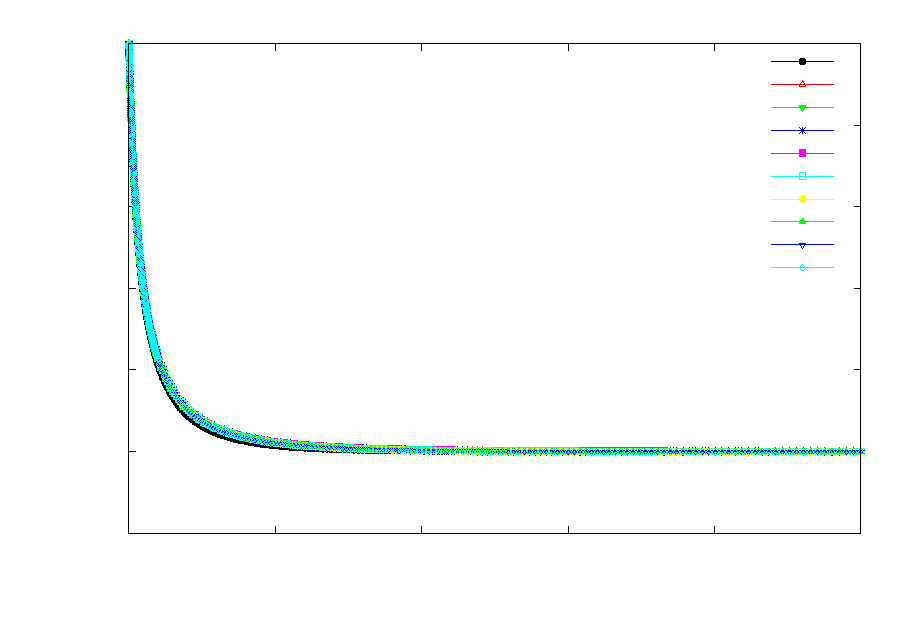
\includegraphics{formfactor}}%
    \gplfronttext
  \end{picture}%
\endgroup

	\caption{Form factor for different $\Lambda$, nx=20}
	\label{fig:formfactor}
\end{figure}

\begin{figure}[htbp]
	\input{formfactorsmall.tex}
	\caption{Form factor for different $\Lambda$ and small momenta, nx=20}
	\label{fig:formfactorsmall}
\end{figure}

\begin{figure}[htbp]
	\input{formfactorbig.tex}
	\caption{Form factor for different $\Lambda$ and big momenta, nx=20}
	\label{fig:formfactorbig}
\end{figure}


Overall, the form factor seems to be exponentially decreasing, and at small momenta almost no difference is visible between the different $\Lambda$. There is a very slight splitting up visible going towards larger momenta. At bigger momenta, the form factor is a lot smaller and so the relative differences are a lot bigger and clearly visible. Going from largest to smallest momentum, the form factor first gets larger, up until the maximum at $\Lambda=500\si{\mega\electronvolt}$, and falls after that, corresponding to the behaviour of the radius. 

\newpage
\listoffigures
\listoftables
\printbibliography
\end{document}
